\section{Hamming码}
\label{sec:ccode-hamming}

引理~\ref{lem:ccode-columns}说，只要校验矩阵的各列非零且互不相同，码就能纠正任意一个翻转。校验矩阵有$r=n-k$行时，非零的列向量一共只有$2^{r}-1$个，所以块长至多为$2^{r}-1$。把它们全部用上，就在给定的冗余位数下得到最长、码率最高的纠单错码，这就是\term{Hamming码}（Hamming code）。$r=3$时，$n=7$，$k=4$，这正是本章开头要找的码：用$7$次信道发送$4$个比特，任何一位翻转都能改回来。

\paragraph{校验矩阵与校验位置}
把$7$个非零的三维列向量按“第$j$列是$j$的二进制表示”排列，最上面一行是最低位：
\begin{equation}
 \bm{H}_7=\begin{pmatrix}
 1&0&1&0&1&0&1\\
 0&1&1&0&0&1&1\\
 0&0&0&1&1&1&1
 \end{pmatrix} .
 \label{eq:ccode-hamming-h}
\end{equation}
例如第$5$列是$(1,0,1)^{\top}$，自下而上读作$101$，正是二进制的$5$。三行分别要求位置$\{1,3,5,7\}$、$\{2,3,6,7\}$、$\{4,5,6,7\}$上的比特之和为偶数。

第$1$、$2$、$4$列是单位向量，各自只出现在一条校验中。可以让这三个位置专门承担校验，其余位置$3,5,6,7$放消息比特$u_1,u_2,u_3,u_4$。每条校验恰好含一个校验位置，于是校验位由消息位直接算出：
\begin{equation}
 c_1=c_3+c_5+c_7,\qquad c_2=c_3+c_6+c_7,\qquad c_4=c_5+c_6+c_7 .
 \label{eq:ccode-hamming-parity}
\end{equation}
这与系统形式只差一个坐标排列：消息仍然原样出现在码字中，只是不在最前面。$\bm{H}_7$的秩为$3$（它含三个单位列），所以码空间的维数是$7-3=4$，码率为$\tfrac47$。

\paragraph{编码一条消息}
取消息$\bm{u}=1011$，放入位置$3,5,6,7$：
\[
 c_3=1,\qquad c_5=0,\qquad c_6=1,\qquad c_7=1 .
\]
由式~\eqref{eq:ccode-hamming-parity}算三个校验位：
\[
 c_1=1+0+1=0,\qquad c_2=1+1+1=1,\qquad c_4=0+1+1=0 .
\]
按位置顺序排好，码字是
\[
 \bm{c}=0110011 .
\]
对四个单位消息分别编码，得到生成矩阵的四行，它们满足$\bm{G}_7\bm{H}_7^{\top}=\bm{0}$：
\[
 \bm{G}_7=\begin{pmatrix}
 1&1&1&0&0&0&0\\
 1&0&0&1&1&0&0\\
 0&1&0&1&0&1&0\\
 1&1&0&1&0&0&1
 \end{pmatrix} .
\]
上面的码字也等于第$1$、$3$、$4$行之和，与式~\eqref{eq:ccode-encode}一致。

\paragraph{最小距离}
$\bm{H}_7$的各列非零且互不相同，由引理~\ref{lem:ccode-columns}，$d_{\min}\geq3$。第$1$、$2$、$3$列之和为零，对应重量为$3$的码字$1110000$，所以$d_{\min}=3$，这是$[7,4,3]$码。枚举全部$16$条码字，重量分布是：重量$0$一条，重量$3$七条，重量$4$七条，重量$7$一条。由定理~\ref{thm:ccode-detect-correct}，它保证纠正一个翻转、检测两个翻转。

\paragraph{单个翻转的定位}
设第$j$位被翻转，$\bm{e}$只在位置$j$为$1$。由式~\eqref{eq:ccode-syndrome-error}，综合征是$\bm{H}_7$的第$j$列，也就是$j$的二进制表示。所以接收端算出综合征，自下而上读成二进制数，就直接得到出错的位置；综合征为零则没有可纠正的错误。不需要查表，对照表已经由列的排列方式给出。

\paragraph{完整核对一次纠错}
发送上面的码字$0110011$，信道翻转第$5$位，收到
\[
 \bm{y}=0110111 .
\]
三条校验依次为
\[
 \begin{aligned}
 s_1&=y_1+y_3+y_5+y_7=0+1+1+1=1 ,\\
 s_2&=y_2+y_3+y_6+y_7=1+1+1+1=0 ,\\
 s_3&=y_4+y_5+y_6+y_7=0+1+1+1=1 .
 \end{aligned}
\]
自下而上读作$s_3s_2s_1=101$，即位置$5$。把第$5$位翻回来得到$0110011$，读出位置$3,5,6,7$上的$1,0,1,1$，恢复消息$1011$。

图~\ref{fig:ccode-hamming-venn}(a)把三条校验画成三个圆：第$i$个圆包含二进制表示中第$i$位为$1$的位置，每个圆内的比特之和必须为偶数。七个位置恰好占据三圆划出的七块区域，校验位$1,2,4$各在只属于一个圆的区域里。翻转第$5$位后，检验$1$与检验$3$不通过，检验$2$通过；同时在圆$1$和圆$3$内、不在圆$2$内的区域只有一块，就是位置$5$。图(b)是同一件事的矩阵读法：综合征$(1,0,1)^{\top}$等于$\bm{H}_7$的第$5$列。

\begin{BookInlineFigure}
 \centering
 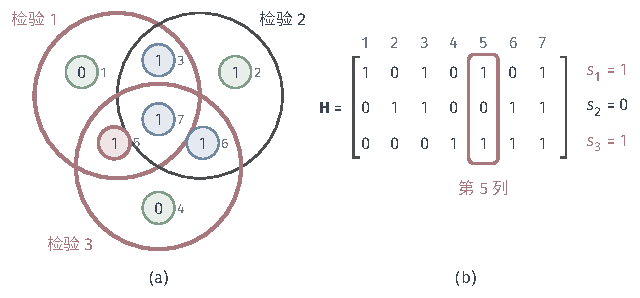
\includegraphics[width=108.3mm]{figures/07-probability/06-channel-coding/tikz/ccode-hamming-venn/figure.pdf}
 \caption{$[7,4,3]$ Hamming码的单错定位。(a) 三个圆是$\bm{H}_7$的三条校验，圆内比特之和应为偶数；小圆中的数是接收块$0110111$各位的值，旁边的小字是位置，绿色为校验位，蓝色为消息位，红色为被翻转的第$5$位。红色粗圆是不通过的检验。(b) 校验矩阵$\bm{H}_7$，第$j$列是$j$的二进制表示（自下而上读）；综合征$(s_1,s_2,s_3)=(1,0,1)$等于红框中的第$5$列。}
 \label{fig:ccode-hamming-venn}
\end{BookInlineFigure}

\paragraph{一个也不浪费}
半径为$1$的Hamming球含$1+7=8$个长度为$7$的串，$16$个码字的球互不相交，合计
\[
 16\times8=128=2^{7}
\]
个串，恰好铺满全部接收块。所以每个接收块都与唯一一条码字相距不超过$1$；$8$个综合征恰好对应“无错”和$7$个单错位置，没有一个综合征被浪费。代价也随之而来：两个翻转一定被“纠正”成第三个翻转。例如两位翻转$\bm{e}$的综合征是两列之和，它等于另一列，译码器会翻转那一位，结果与原码字相差三位。

\paragraph{与重复码对比}
Hamming码与三次重复码的最小距离都是$3$，都保证纠正一个翻转，但保证的范围不同。三次重复码在每$3$次使用中纠正一个翻转，每个消息比特各有自己的保护；Hamming码在$7$次使用中只纠正一个翻转，四个消息比特共享这份保护。前者码率$\tfrac13$，后者码率$\tfrac47\approx0.571$。

在$p=0.1$时，Hamming码的块错误概率是至少两位翻转的概率：
\[
 P_{\mathrm{e}}=1-0.9^7-7\times0.1\times0.9^6=1-0.47830-0.37201=0.14969 .
\]
三次重复码发送同样$4$个比特的块错误概率约为$0.107$，不编码时为$0.344$。逐个比特看，对$128$个错误向量逐一枚举综合征译码的结果，Hamming码的比特错误率是$0.0669$，三次重复码是$0.028$，不编码是$0.1$。

图~\ref{fig:ccode-hamming-ber}把比较延伸到不同的翻转概率。$p$较小时，两种码的比特错误率都与$p^2$同阶，因为都需要两个翻转才出错；Hamming码的系数更大，因为$7$位中出现两个翻转的方式比$3$位中多。$p=0.01$时，Hamming码的比特错误率为$8.7\times10^{-4}$，三次重复码为$3.0\times10^{-4}$。Hamming码用略高的错误换取了高得多的码率。

\begin{BookInlineFigure}
 \centering
 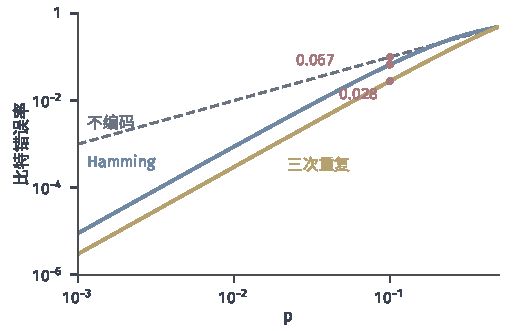
\includegraphics[width=88mm]{figures/07-probability/06-channel-coding/matplotlib/ccode-hamming-ber/figure.pdf}
 \caption{二元对称信道上的比特错误率随翻转概率$p$的变化，双对数坐标，均为精确值：不编码（灰色虚线，码率$1$），$[7,4,3]$ Hamming码配合综合征译码（蓝，码率$\tfrac47$，对$128$个错误向量逐一枚举），三次重复码配合多数判决（黄，码率$\tfrac13$）。红点为$p=0.1$处的值。}
 \label{fig:ccode-hamming-ber}
\end{BookInlineFigure}

\paragraph{有限构造不是容量的证明}
在$p=0.1$的信道上，Hamming码的码率$0.571$已经超过容量$0.531$。这并不矛盾：容量限制的是错误能否趋于零，单个有限码的错误概率$0.15$并不为零。同一族中更长的Hamming码码率更高，$r$个校验位对应码率
\[
 \frac{2^{r}-1-r}{2^{r}-1}\to1 ,
\]
但每个块只保证纠正一个翻转。块长$n$增大时，$n$个位置中至多一个翻转的概率$(1-p)^{n}+np(1-p)^{n-1}$趋于零，所以对固定的$p>0$，块错误概率趋于$1$。要让错误趋于零而码率保持为正，能纠正的翻转数必须随块长按比例增长，Hamming码族做不到这一点。它是一个结构清楚、译码极其简单的有限构造，不能当作渐近达到容量的例子。
